\documentclass[a4paper]{article}

\usepackage{graphicx}
\usepackage{float}
\usepackage[margin=3cm]{geometry}

\graphicspath{{images/}}

%opening
\title{koda: Deep Learning-Enhanced Pipeline for Keyword Detection in Document Images} 
\author{Matteo Pellegrino, Federico Terzi}

\begin{document}

\maketitle

\begin{abstract}
TODO
\end{abstract}

\section{Introduction}
TODO


\section{Edge Detection}

Above all the possible approaches, the pipeline proposed in this paper heavily
relies on edges to detect documents inside images. Therefore, in order to obtain
good results, it is crucial to employ a solid \textit{edge detection} algorithm.


\subsection{First Attempts with Canny}

Our initial attempts to detect document edges involved the well known \textit{Canny edge detector} [TODO REF]. Although applying the filter directly does detect the sheet edges, it presents many artifacts
due to the text printed on the document itself (as seen in Fig. \ref{fig:canny_gaussian} (B)).

In order to mitigate the problem, a \textit{Gaussian filter} [TODO REF] is applied before the edge detection, obtaining a clear highlighting of the interesting edges (as seen in Fig.  \ref{fig:canny_gaussian} (C)).

\begin{figure}[!htb]
	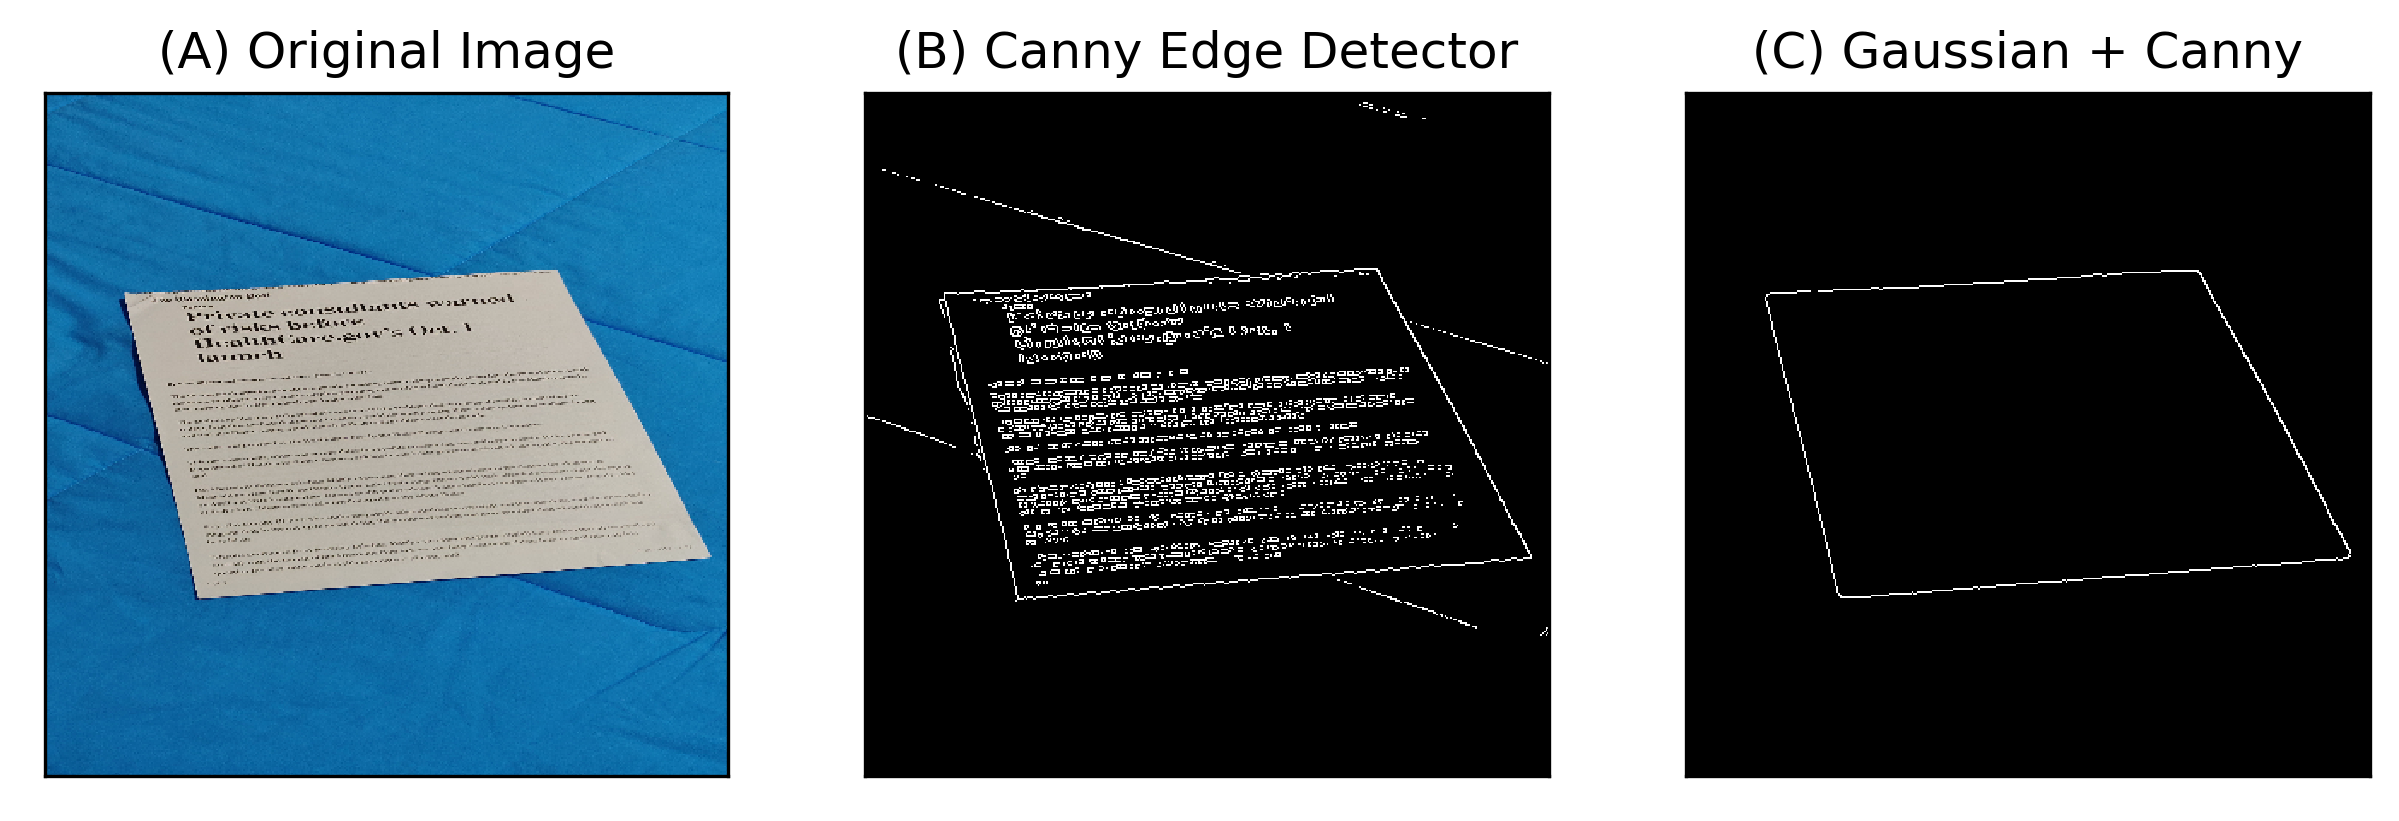
\includegraphics[width=\linewidth]{canny_gaussian.png}
	\caption{TODO}
	\label{fig:canny_gaussian}
\end{figure}

Despite the result, after many observations it became clear that this approach was not robust enough to
work in all real-world scenarios. In particular, Canny's parameter tuning turned out to be a major
problem, as it can be seen in Fig \ref{fig:canny_comparison}, where a combination of parameters,
despite producing good results in some scenarios, proved itself incapable of generalizing well in others.

\begin{figure}[htb!]
	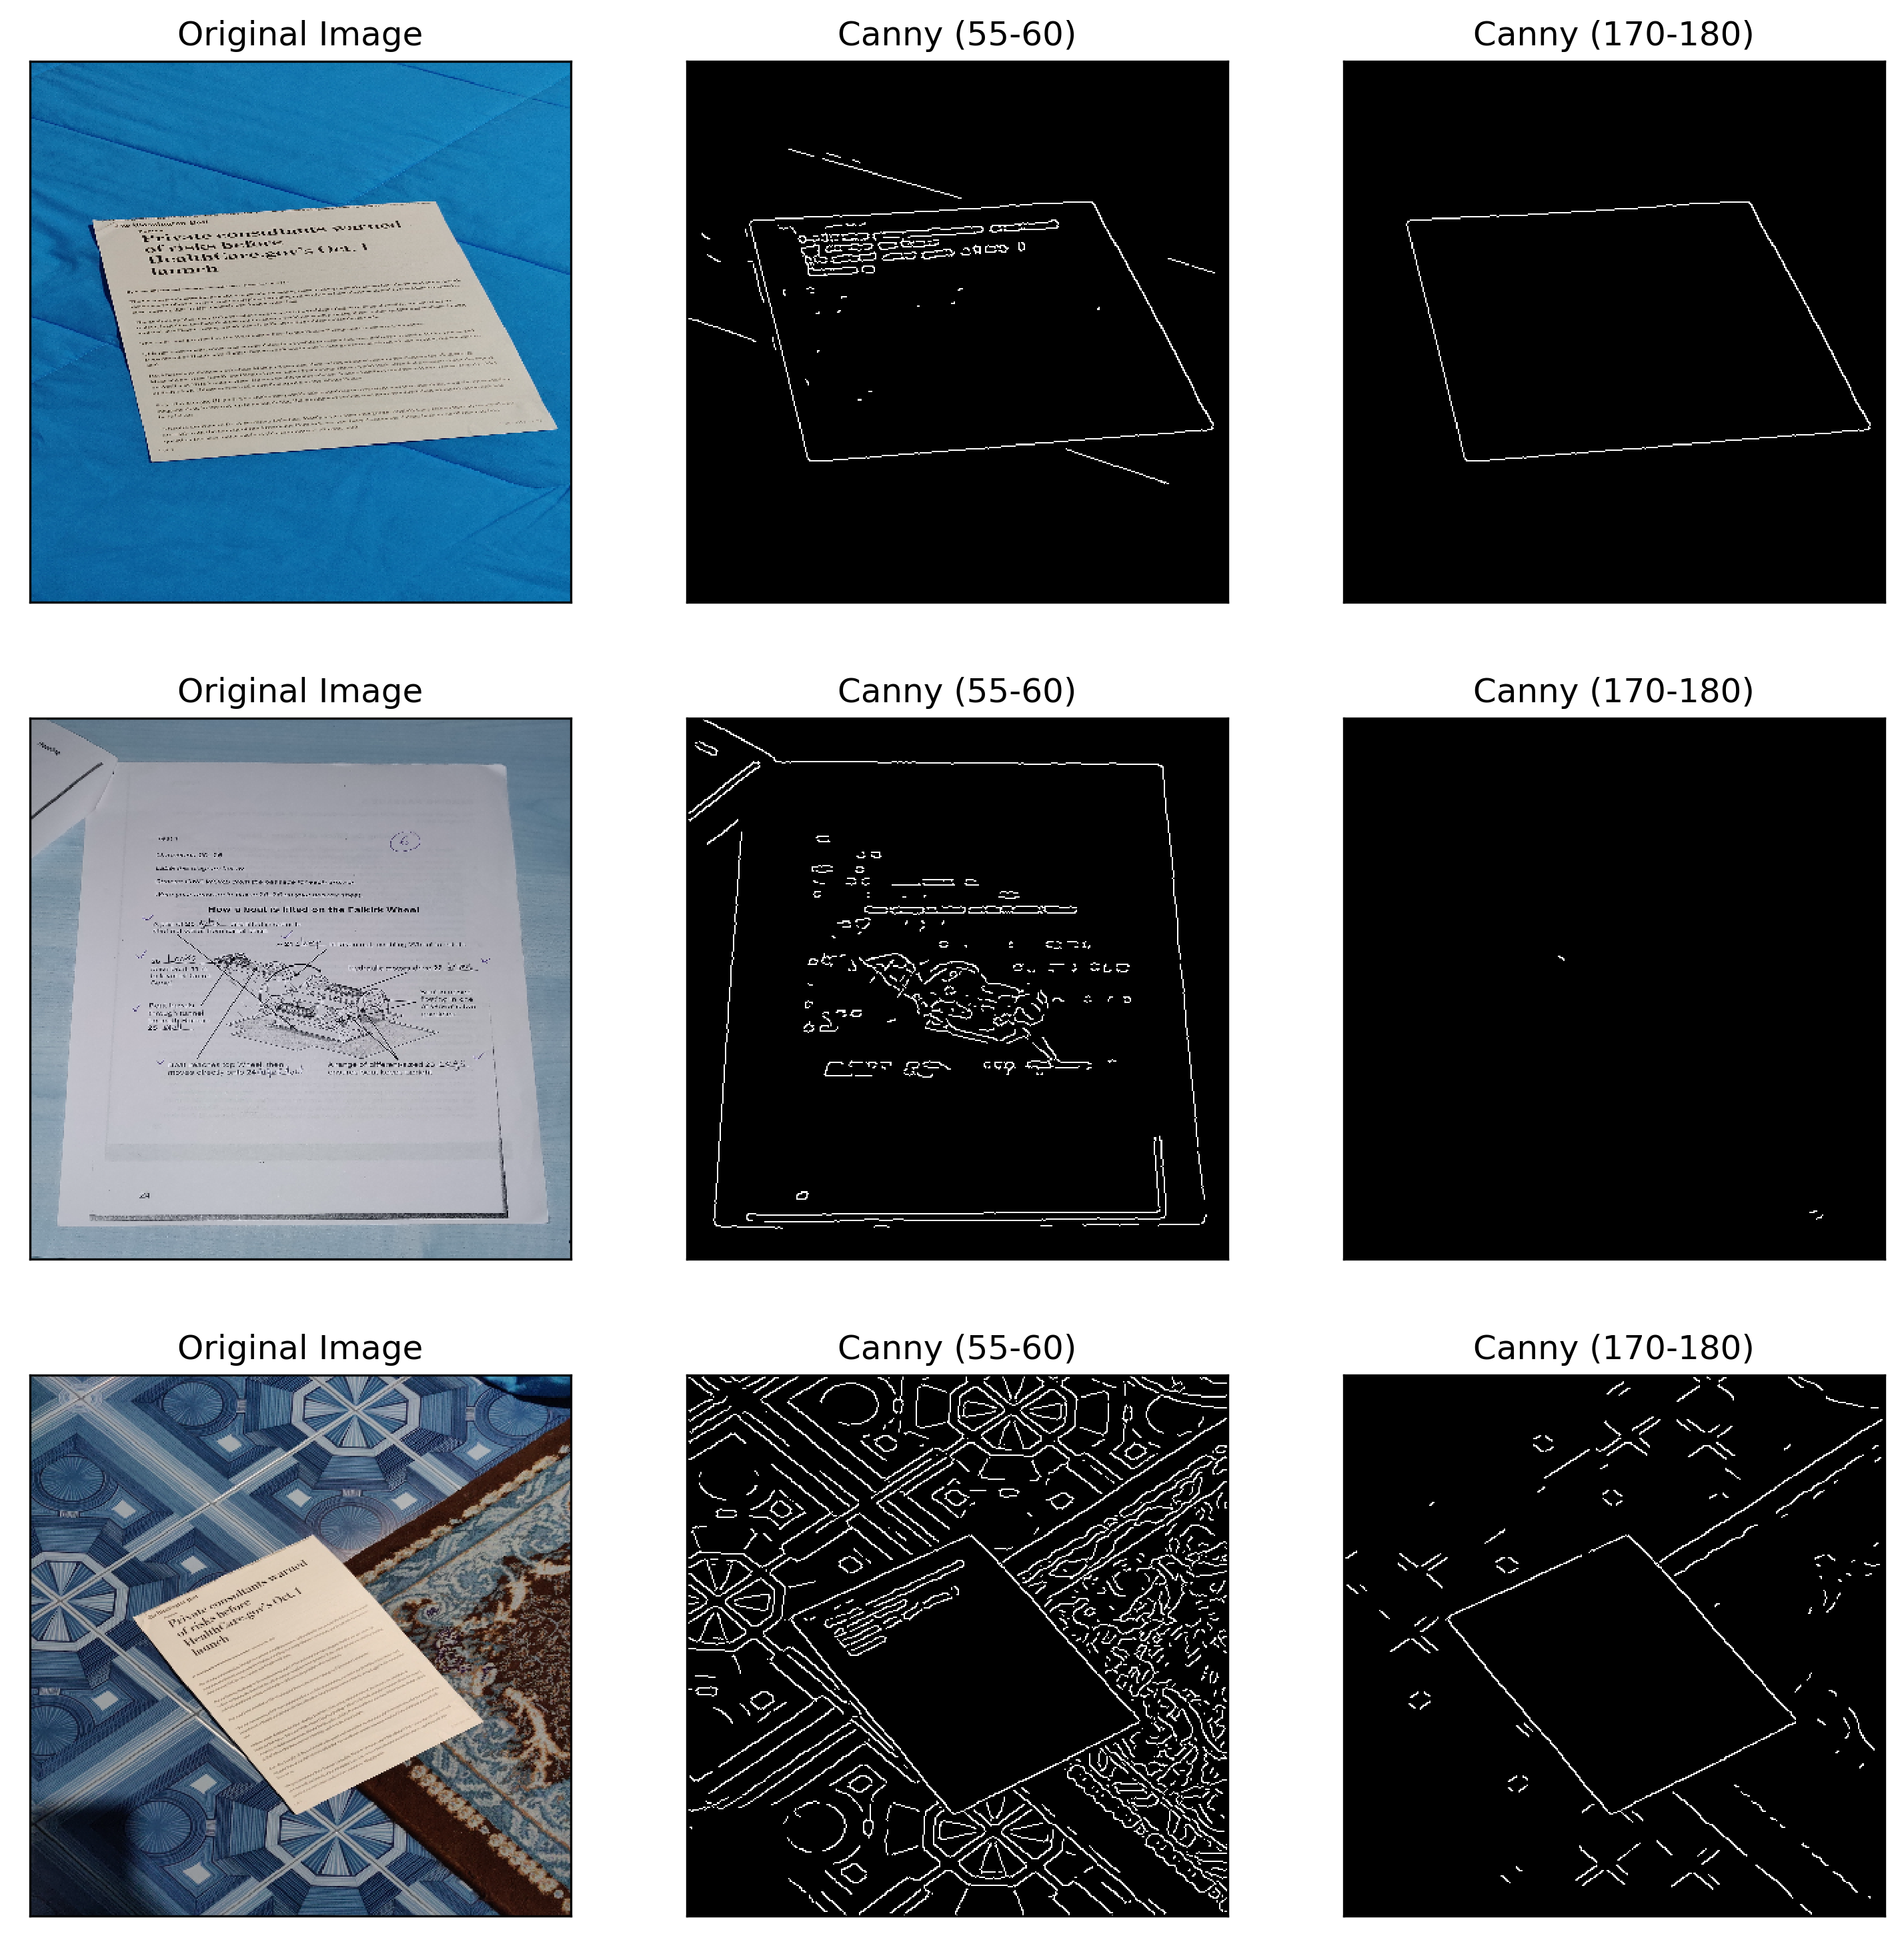
\includegraphics[width=\linewidth]{canny_comparison.png}
	\caption{TODO}
	\label{fig:canny_comparison}
\end{figure}

\subsection{Deep Learning Approach}

In order to make the pipeline able to deal with real-world images, it is crucial to develop an
edge detection mechanism capable of generalizing better in heterogeneous situations. 
For this reason, a \textit{Deep Learning}-based approach was explored with the aim of creating a model
capable of distinguishing document sheet edges from the rest of the image.

Due to the lack of a suitable dataset with labelled document edges, a custom one was created.
In particular, 250 images containing document sheets were taken under different lighting conditions, 
backgrounds and positions. Thereafter, every image was labelled with the 4 corner coordinates of the document.

For this particular task, \textit{Keras}, an open-source Python library for Deep Learning [TODO REF], was chosen to build the model. Many experiments were made to find the right architecture, most of them 
exploiting \textit{convolutional neural networks}. Above all of them, KODA uses \textit{U-Net}[TODO REF], a popular architecture for \textit{object segmentation}, and in particular an open-source implementation for Keras [TODO REF].

The model takes a 3-dimensional input image (RGB) and outputs a 2-d map of the edges. Although the shape
of those matrices can vary, KODA uses a 256 pixels side for both input and output, as it provides a reasonable compromise between size and resolution. Fig. \ref{fig:label_edge} illustrates the way a
sample is fed to the network. In particular, the input image is resized to a 256x256 RGB image and the
output label is a gray scale map of the expected document edges.

\begin{figure}[htb!]
	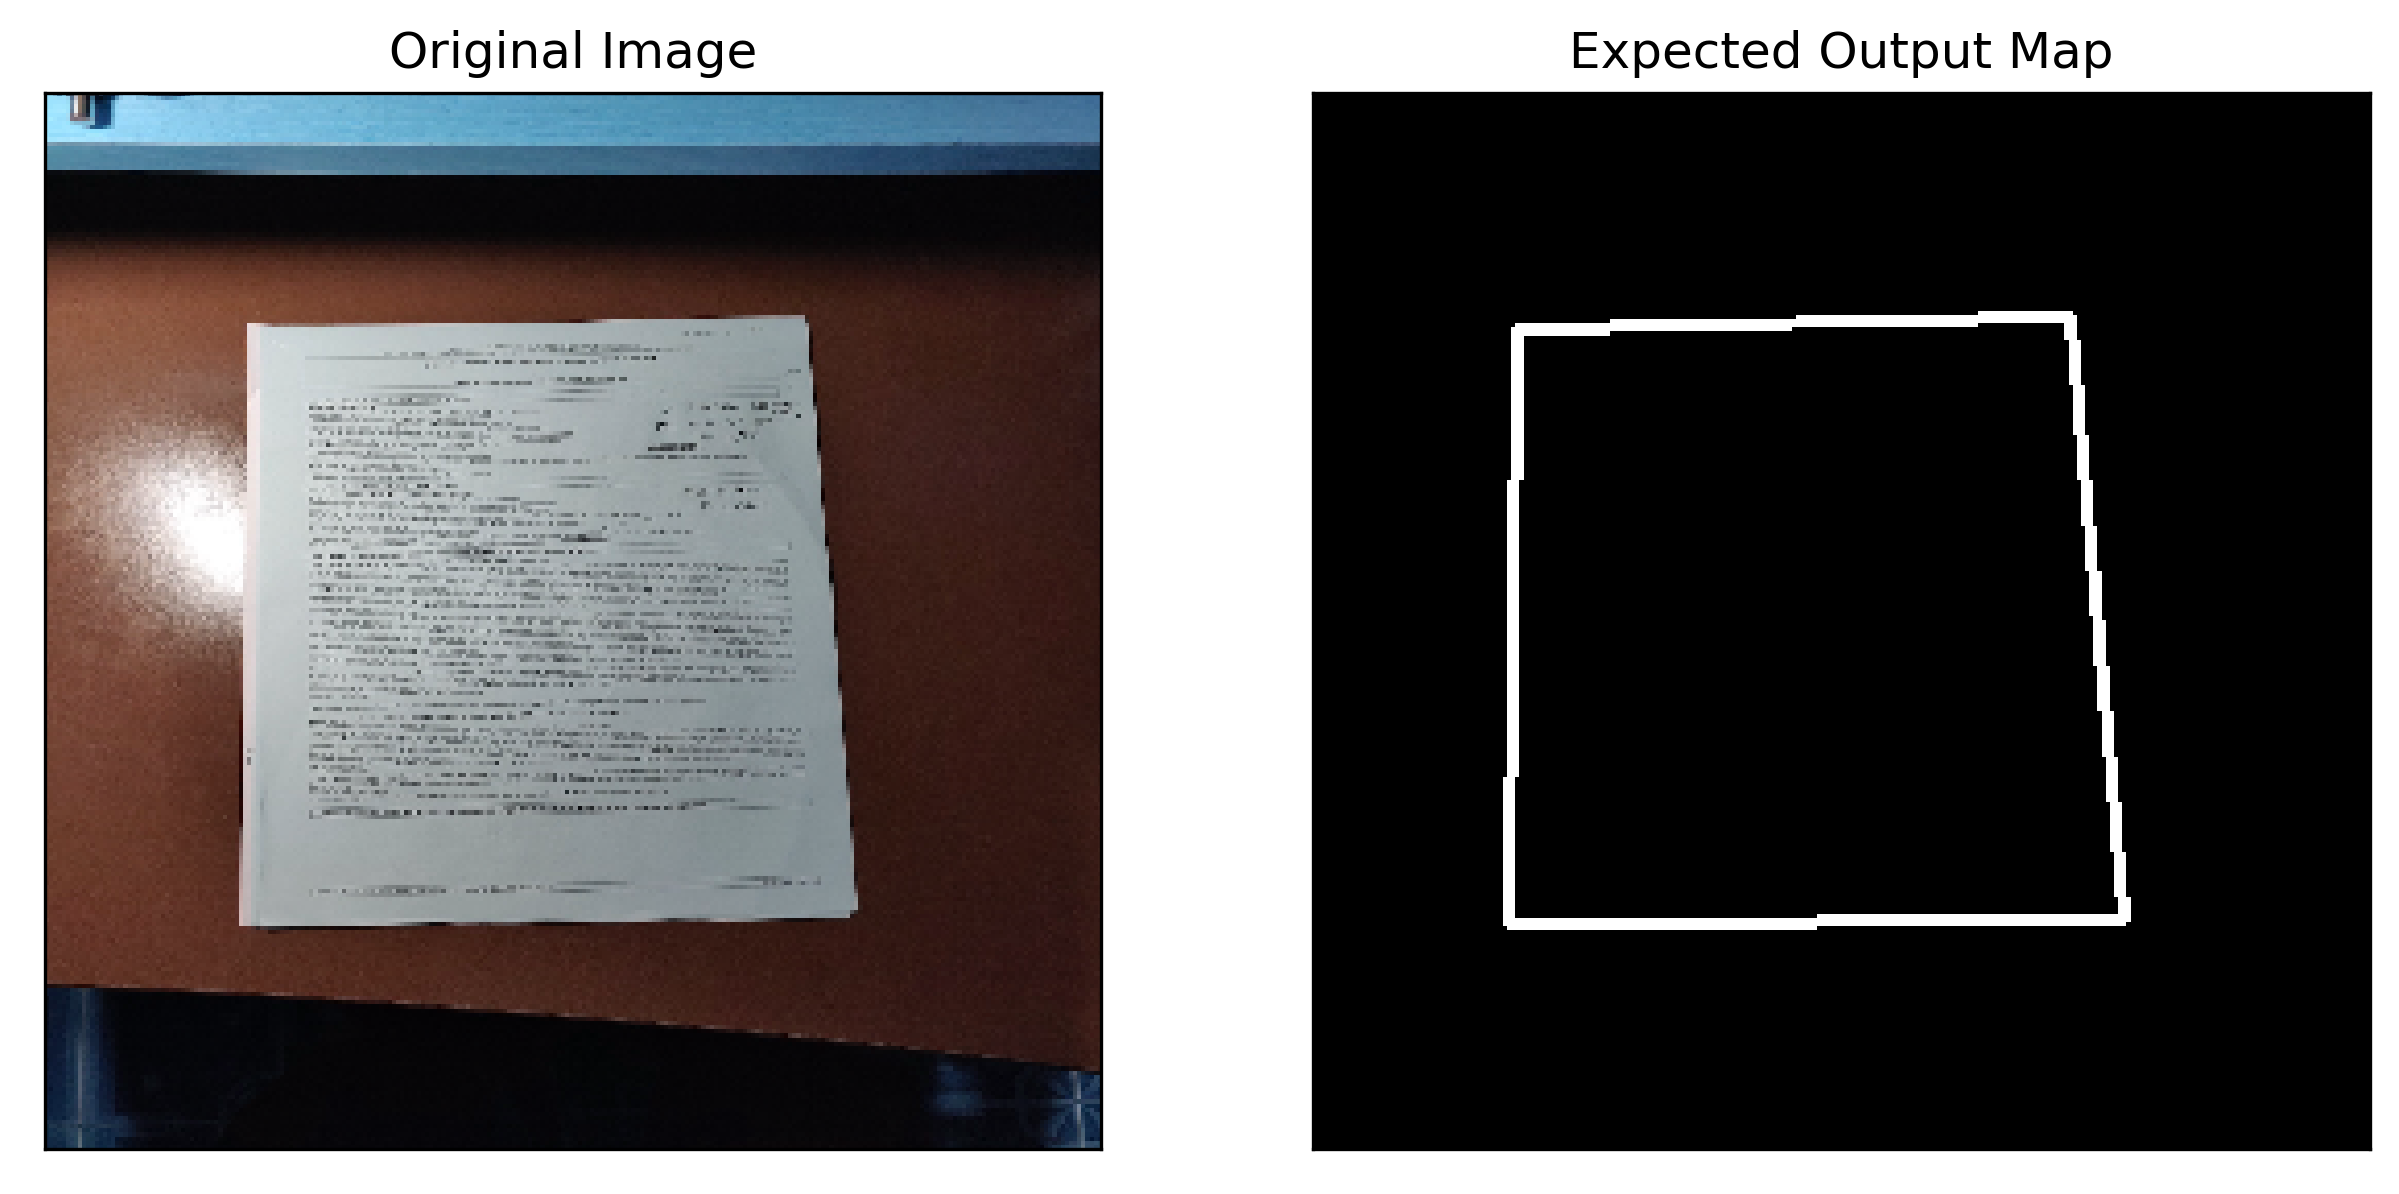
\includegraphics[width=\linewidth]{label_edge.png}
	\caption{Example of the way a sample is fed to the network.}
	\label{fig:label_edge}
\end{figure}

Due to the high number of required samples, the dataset itself is insufficient to fully train the network.
For this reason, a technique called \textit{data augmentation}[TODO REF] is applied to provide the model
with enough variability. In particular, before being fed to the network, a random combination of transformations, such as scale, translation, rotation and brightness changes, is applied to the image and to the resulting edge feature map, as shown in Fig. \ref{fig:augmented_image}.

\begin{figure}[H]
	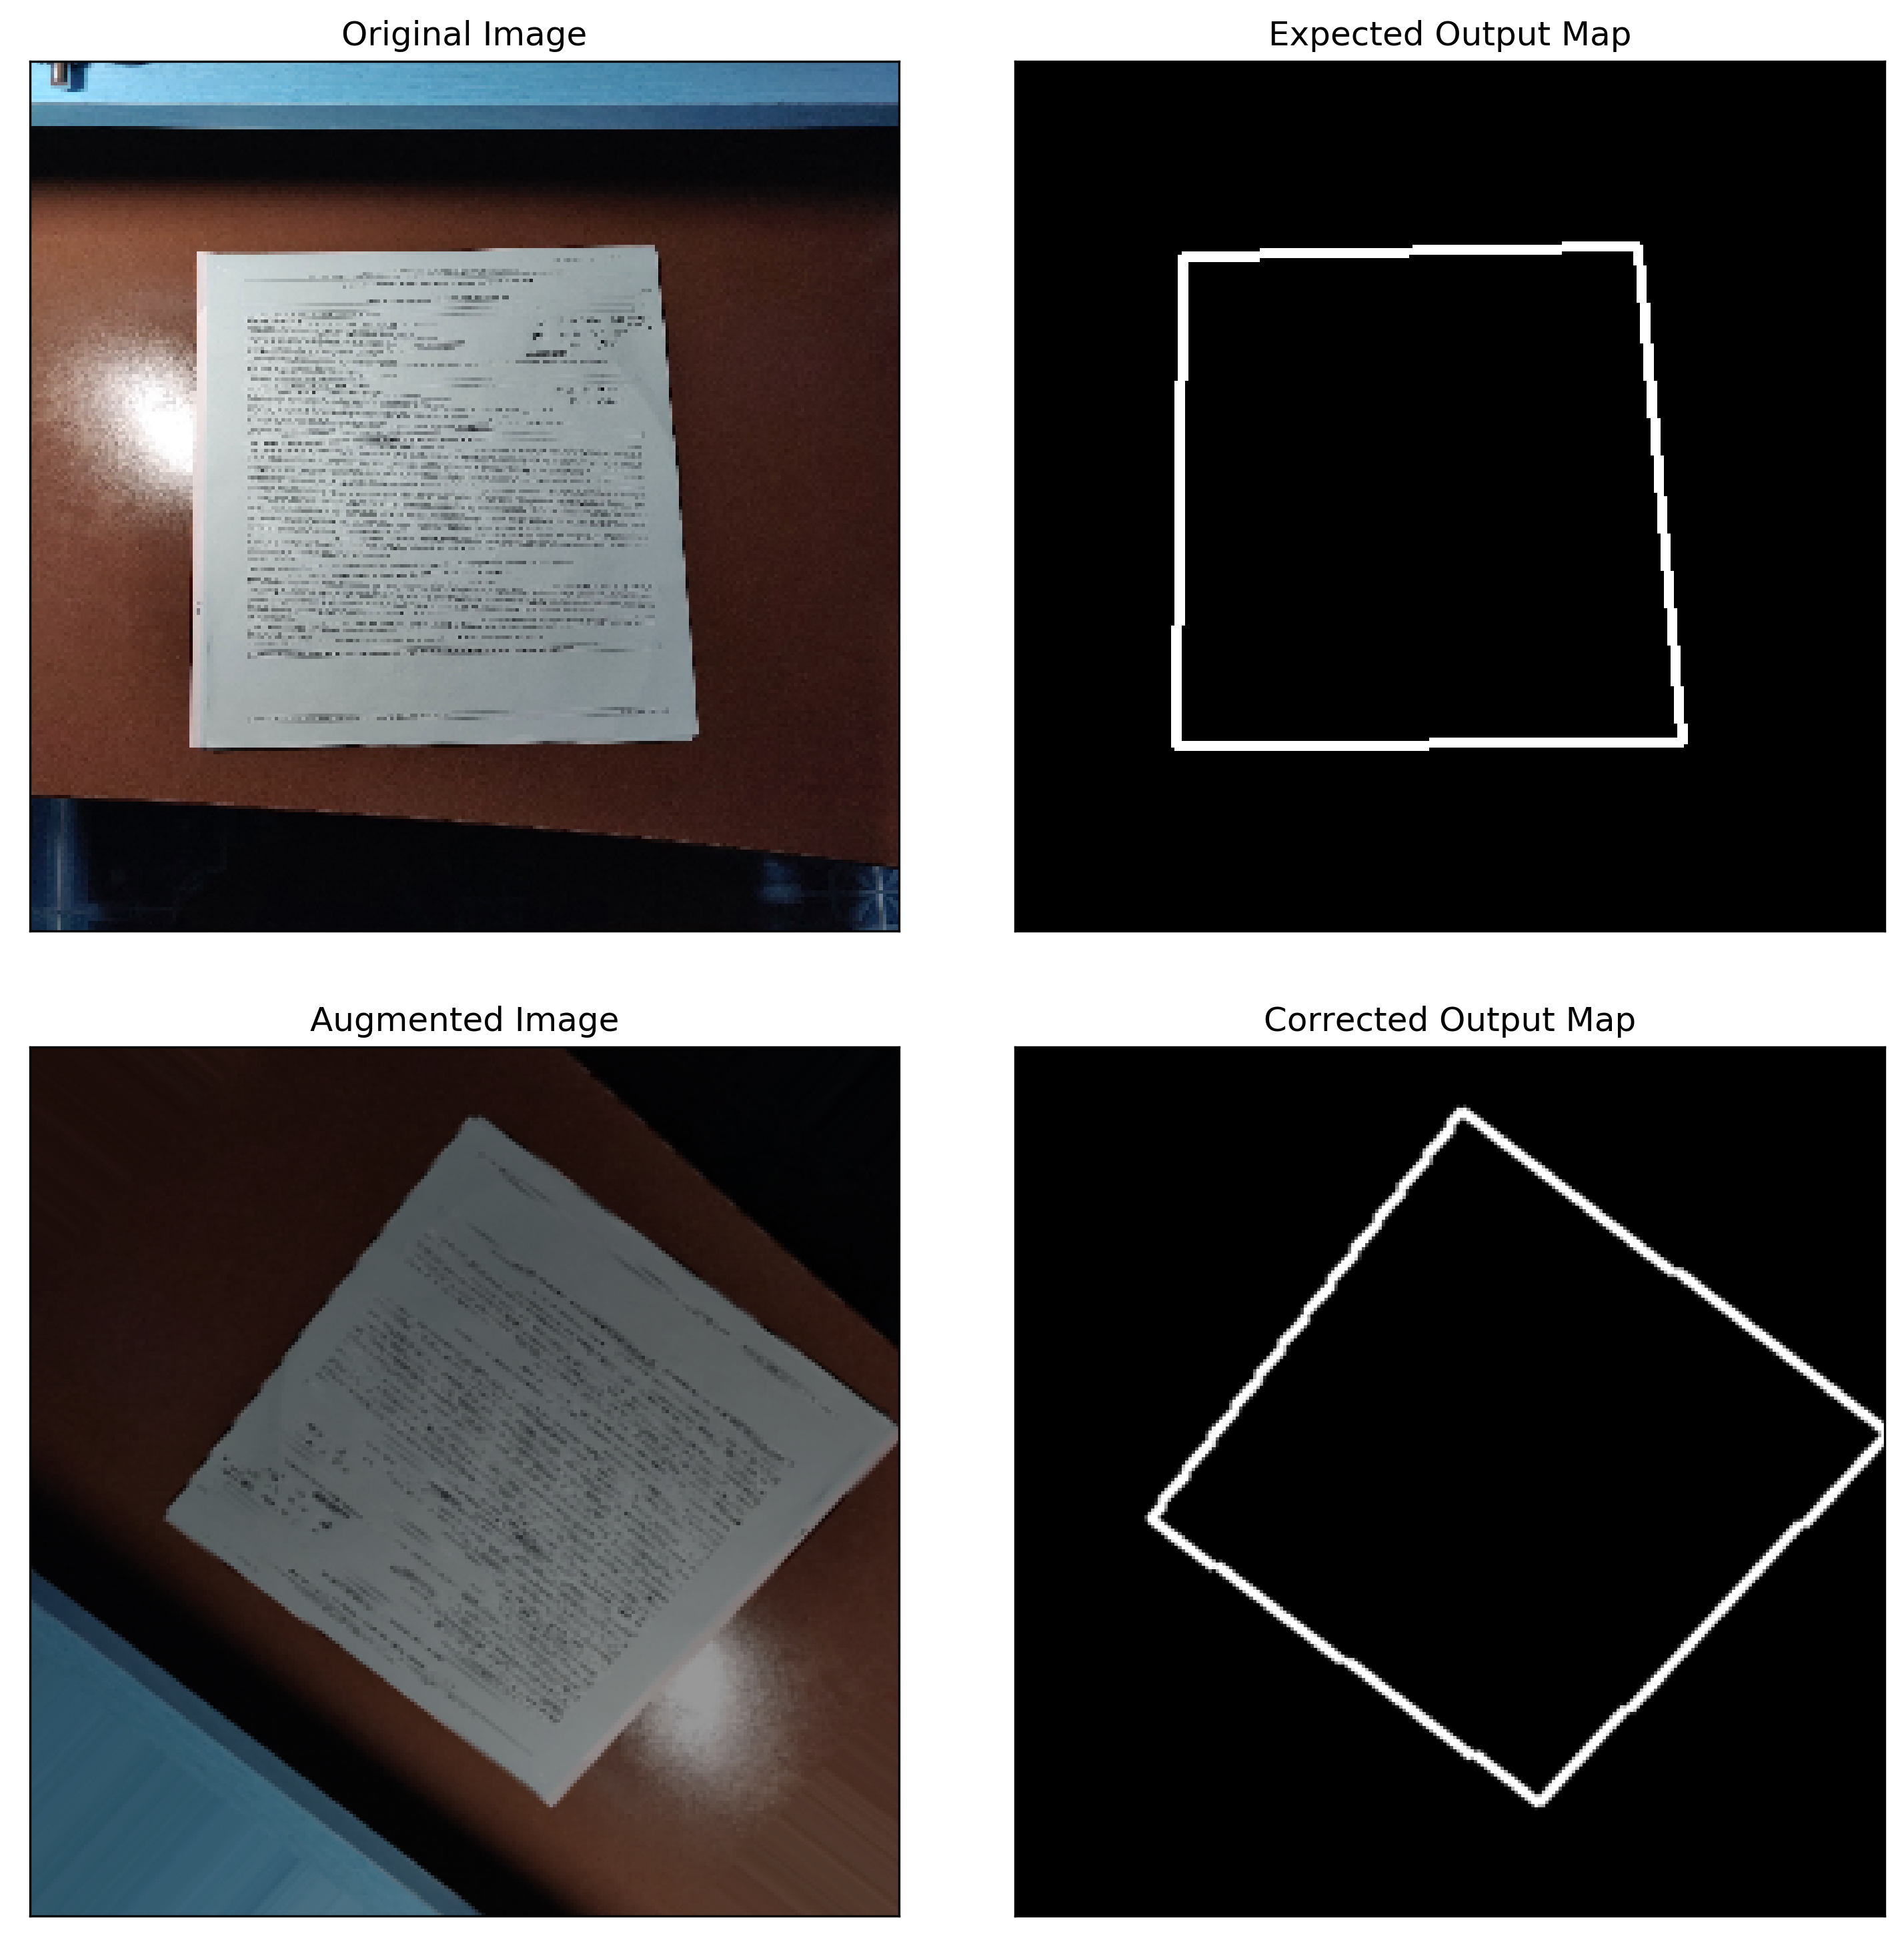
\includegraphics[width=\linewidth]{augmented_image.png}
	\caption{Example of Data Augmentation}
	\label{fig:augmented_image}
\end{figure}

During the training, finding the best compromise between good results and overfitting proved to be a challenging problem. In particular, the \textit{loss function}, in this case \textit{binary crossentropy}, 
was not representative of the model's quality. As it can be seen in Fig. \ref{fig:model_loss}, the loss value of the validation set settles around epoch 40. Despite this, further experimentation shows that the model still improves well beyond that epoch. For this reason, a new approach was needed to evaluate the performances of the model.

\begin{figure}[htb!]
	\centering
	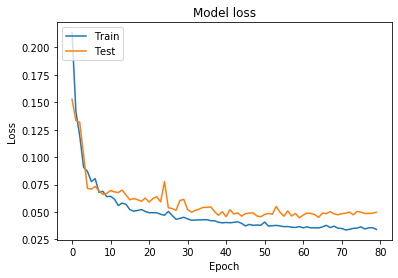
\includegraphics[width=0.7\linewidth]{model_loss.png}
	\caption{Model loss over the first 80 epochs.}
	\label{fig:model_loss}
\end{figure}

Despite being simple, the proposed solution is to save the current model's results over a set of test images after each epoch, as well as saving the model itself. This approach allows a simple comparative analysis, and allowed us to select the best model according to its actual results. Epoch 70 produced the best performing model from a generalization standpoint, while further epochs shown interesting but less effective trends. In particular, as you can see from Fig. \ref{fig:edge_comparison_epoch}, the model at epoch 70 is capable of detecting both (A) and (B) edges fairly well, whereas the one at epoch 140 presented an improved result in (A), removing uninteresting objects from the top portion of the image, but was almost incapable of recognizing edges in (B). This phenomenon could be explained as the model starting to empathize straight lines and discarding curved ones. Unfortunately, the latter are a common case and should be considered, therefore the first model was chosen.

\begin{figure}[htb!]
	\centering
	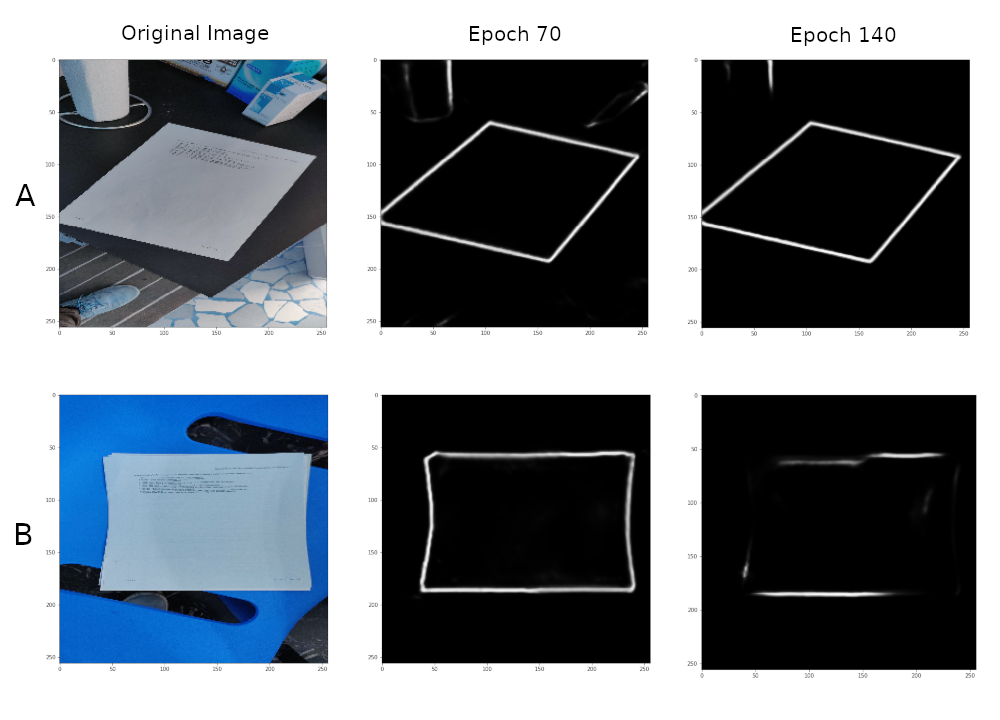
\includegraphics[width=\linewidth]{edge_comparison_epoch.png}
	\caption{Comparison of the edge detector over different epochs.}
	\label{fig:edge_comparison_epoch}
\end{figure}


An overview of the end result can be seen in Fig. \ref{fig:deep_comparison}, which also shows a comparison with the previous Canny-based approach.

\begin{figure}[htb!]
	\centering
	\makebox[\textwidth][c]{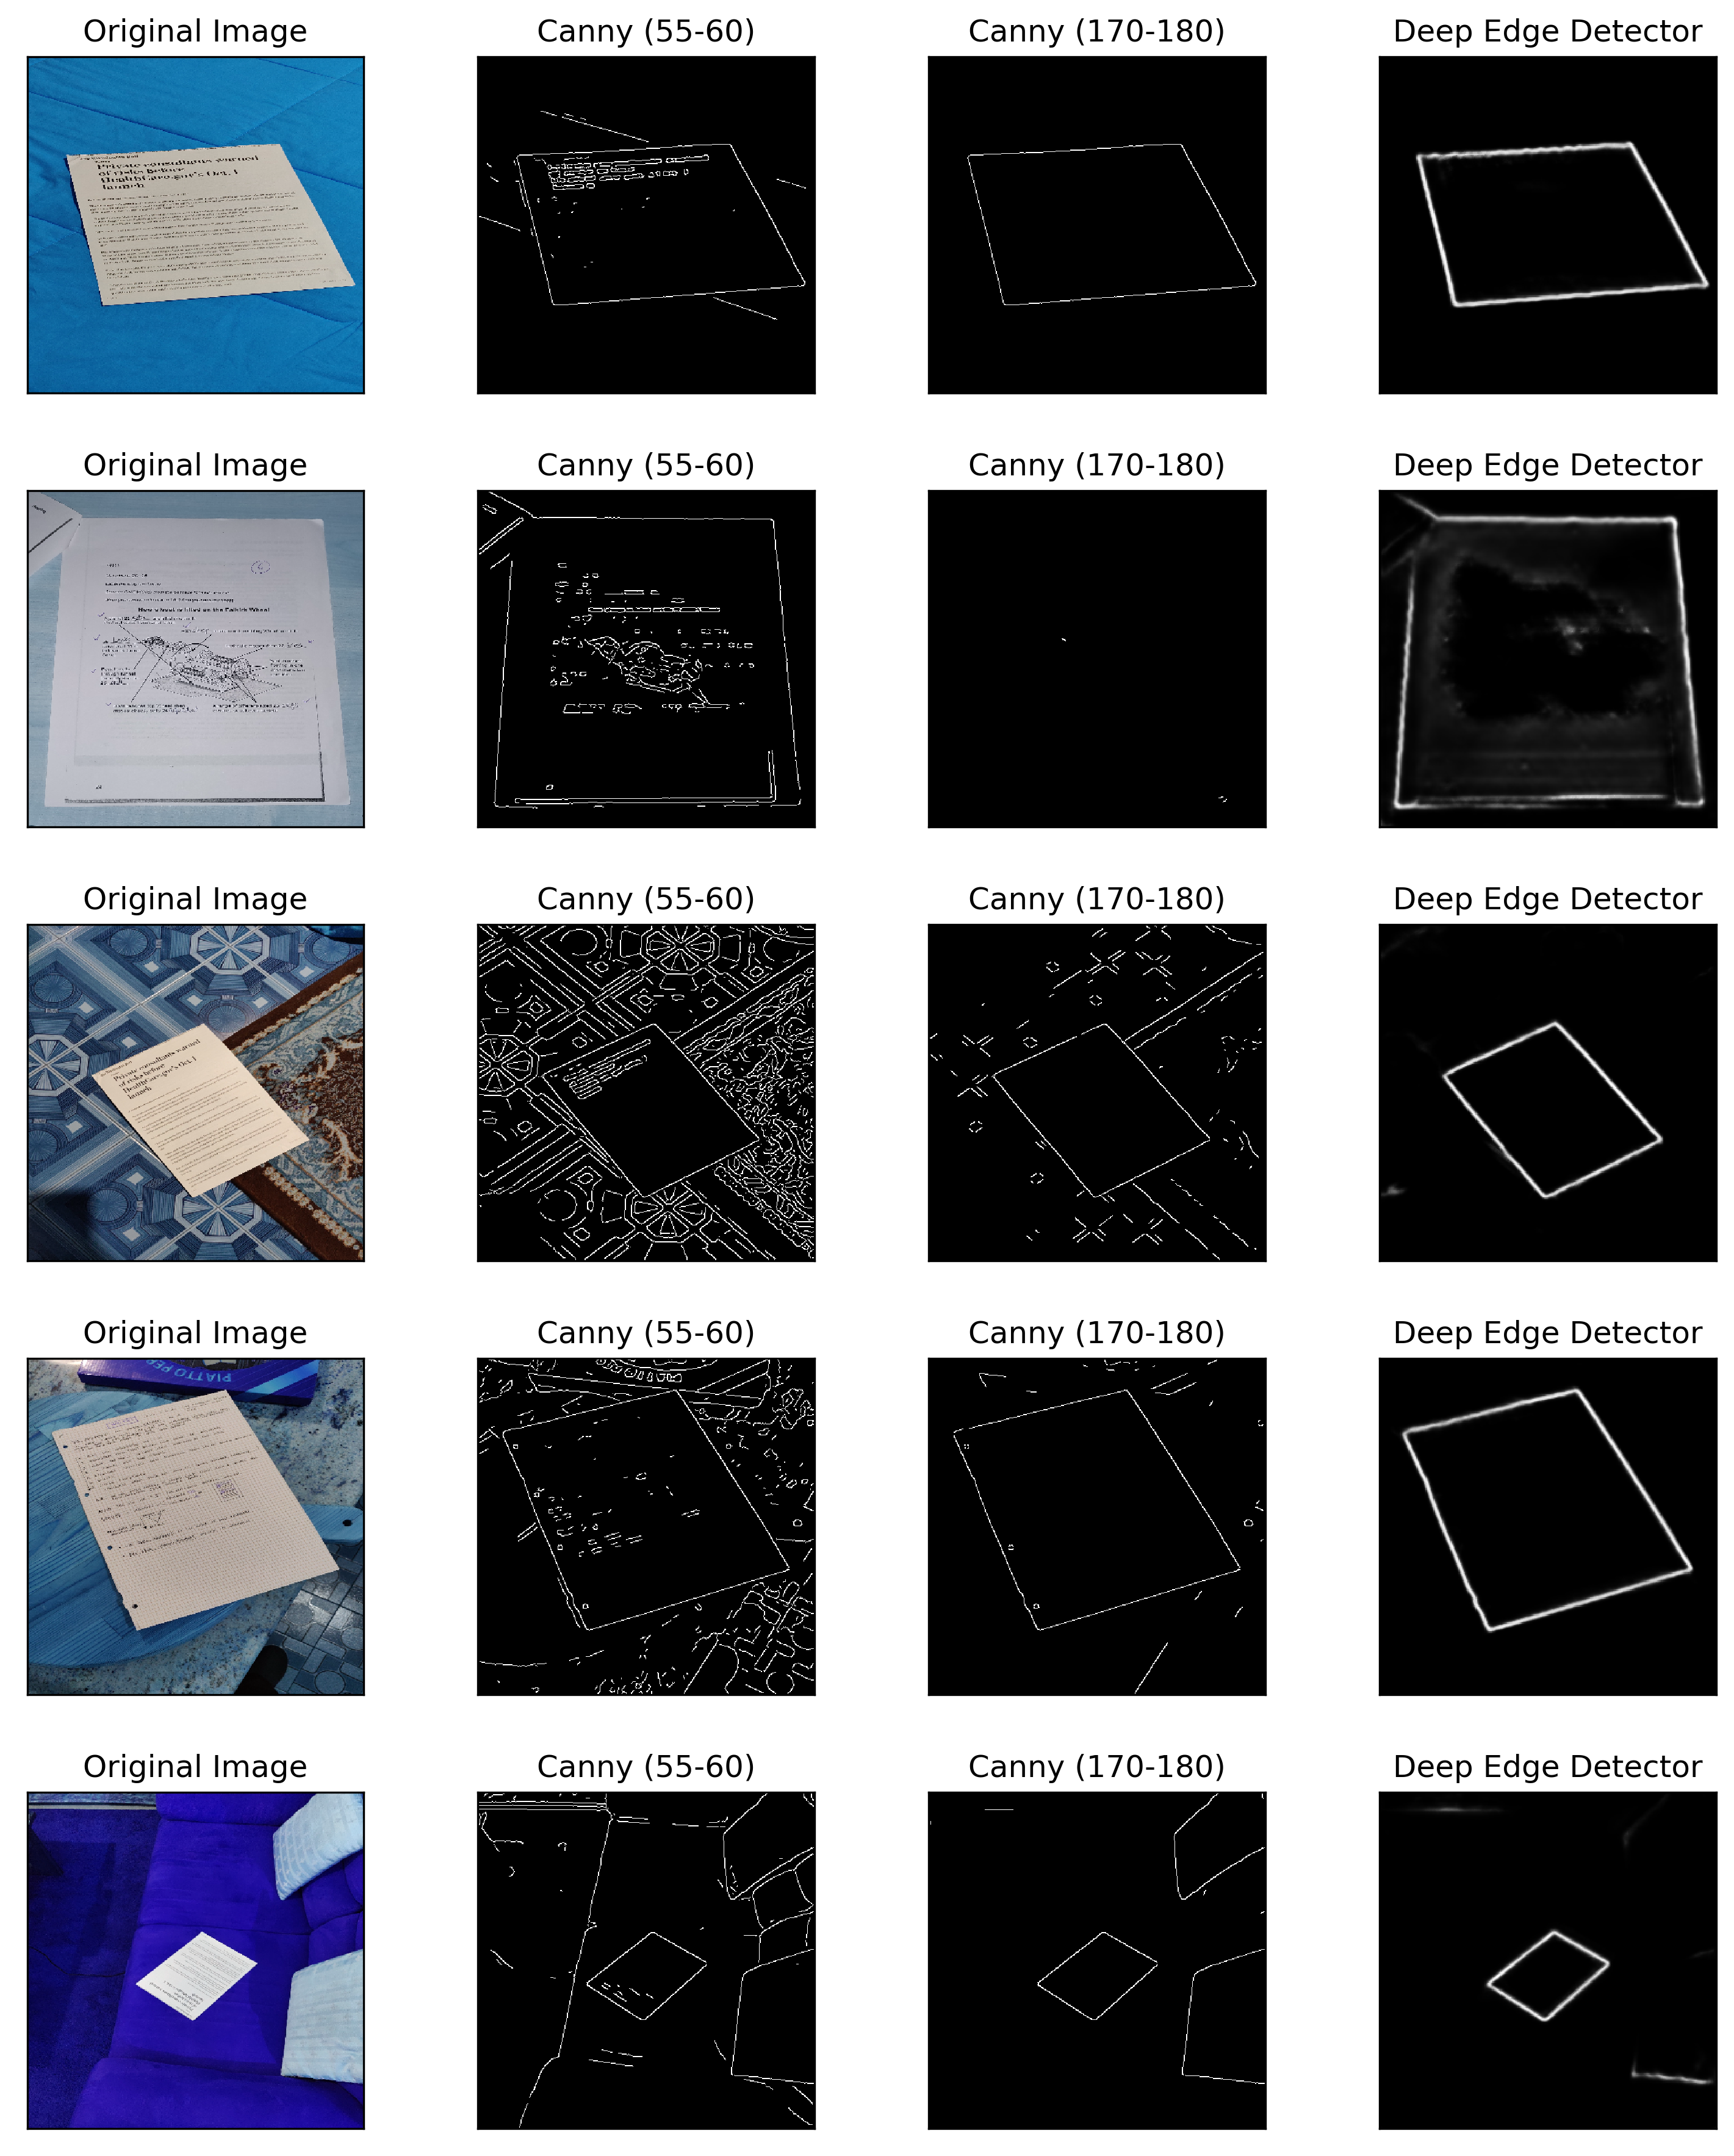
\includegraphics[width=1.2\textwidth]{deep_edge_comparison.png}}%

	\caption{Comparison of Canny and Deep Learning-based edge detection.}
	\label{fig:deep_comparison}
\end{figure}



\end{document}
